\documentclass[10pt,twocolumn,openany,nodeprecatedcode,bg=none,inline]{dndbook}

\usepackage[english]{babel}
\usepackage[singlelinecheck=false]{caption}
\usepackage[,inline]{enumitem}
\usepackage{hyperref}
\usepackage[utf8]{inputenc}
\usepackage{graphicx}


% Don't skip an extra page before mainmatter.
\makeatletter
\renewcommand\mainmatter{\clearpage\@mainmattertrue\pagenumbering{arabic}}
\makeatother

\captionsetup[table]{labelformat=empty,skip=0pt}

\DndSetThemeColor[DmgSlateGray]

\title{\DndFontChapter Lost Mind of Phandelver \\ \DndFontSection \centering Prologue}
\author{\DndFontSubsection Braedy Kuzma}
\date{}

\begin{document}

\frontmatter%

\maketitle

\chapter*{Preface}
This is my party's opening to the Lost Mine of Phandelver adventure.
Instead of being beginning the adventure already on the road protecting the wagon, the party will first be brought together to rescue the map to Wave Echo Cave from a group of thieves in Neverwinter.

Gundren has purchased the map to Wave Echo Cave from a seller in Waterdeep.
As it is being delivered in Neverwinter, the deliveryman and his guard are robbed and lose the map.

Players begin a small set of encounters where they search for the thieves who took the map and eventually confront them in order to retrieve the map.
Upon its return, Gundren will ask them to join him in Phandalin and the adventure will proceed as normal, barring the adventure hook proposed in the adventure.

\tableofcontents

\nopagebreak
\mainmatter%

\chapter{Introduction}
The players and the DM should work together to determine a reason that they
\begin{enumerate*}[label={(\arabic*)}]
  \item find themself in the city of Neverwinter, and
  \item find themself acquainted with any of the three Rockseeker brothers.
\end{enumerate*}

For the purposes of this campaign hook, prompt players with the following background information:
\begin{DndReadAloud}
  Gundren Rockseeker and his two brothers, Nundro and Tharden, are fairly well known smiths in the city of Neverwinter.
  Gundren also happens to deal a bit in antiquities and oddities on the side and has been known to purchase some that catch his eye for a sizeable amount.
  Lately, he's also been looking for information on abandoned ruins in the area of the city, something for which he has also offered some bounty.
  The three brothers also do some charitable work, helping those down on their luck.
  For the more frail, this is sometimes soup and a bed, for the more hardy, they are offered tasks or minor quests in return for pay.
\end{DndReadAloud}

This opening gives hooks for players through the brothers' or specifically Gundren's actions and reputations while leaving both Nundro and Tharden as blank slates for players who want to develop their own stories.

\section{The Hook}
Players will be gathered together in order to retrieve an artifact (the map to Wave Echo Cave) intended for delivery to Gundren Rockseeker, the evening prior.
Read the following aloud to start the events:
\begin{DndReadAloud}
  At roughly midday, a dirty adolescent approaches each of you and offers you a note.
  Turning it over shows a wax seal stamped with the Rockseeker signet which you recognize from the sign hanging above their smithy door.
\end{DndReadAloud}

Each of the messengers has varied age, race, and sex and is recognizeable by every player as one of the children that loiters near the smithy, hoping for small tasks to support their families.
Those whose backstories imply that they are close with the Rockseekers or spend a lot of time in the area may know the messenger by name.
If any of the players tip their messenger or treat them particularly well, have them introduce themself and tell the player that if they ever need something, to go find them.
Keep the messenger's name handy so that they can approach the party at a later time, see \hyperref[sec:investigation]{The Investigation}.
For a list of potential messengers, see the \hyperref[tab:messengers]{Example Messengers} table.

\begin{table}[b]
  \caption{}
  \label{tab:messengers}
  \begin{DndTable}[header=Example Messengers]{cXXXX}
    \textbf{d8} & \textbf{Name} & \textbf{Race} & \textbf{Sex} & \textbf{Age}\\
    1 & Rael & Half-Elf & Female & 17 \\
    2 & Gnok & Darf & Male & 15 \\
    3 & Vellum & Gnome & Female & 11\\
    4 & Lyle & Halfling & Male & 16 \\
    5 & Milly & Human & Female & 13 \\
    6 & Aghrim & Human & Male & 10 \\
    7 & Alys & Human & Female & 14 \\
    8 & Orly & Human & Male & 17
  \end{DndTable}
\end{table}

Once everyone has received their letter, upon opening it, each has a short personalized letter, written in Gundren's own hand with several elements.
It proceeds as follows:
\begin{itemize*}[label={}, itemjoin={;}, after={.}]
  \item a short greeting
  \item a description of how he knows them or came to heard of them and their deeds as an adventurer, mercenary-for-hire, etc.
  \item asks that you join him at the smithy as soon as possible to help him with an issue
\end{itemize*}

Allow players to gather their things and head to the Rockseeker smithy.
Upon arriving, an apprentice watching the storefront directs the players to the office attached to the showroom which is normally reserved for entertaining buyers of large or expensive orders.
Gundren greets them as they enter, and offers them each a seat.
Once everyone is seated, Gundren tells them his story:
\begin{DndReadAloud}
  Thank you for coming everyone.
  I find myself in a spot of trouble and myself or my brothers know each of you to be\dots capable friends.
  I'll get right to it, as it's a matter of some urgency.
  I recently bought an artifact from a rather difficult seller in Waterdeep for quite a hefty sum.
  As it was being delivered -- in fact, shortly after it arrived in the city -- my deliveryman and his guard were accosted and robbed.
  Being outnumbered and fearing for their lives, they were forced to hand over everything.
  I'd like for you to help me -- discretely -- retrieve the small metal coffer that contains my delivery.
  I'm prepared to offer you 10 gold each on its successful return as well as future employment that should prove profitable for the both of us, if you are interested.
\end{DndReadAloud}

If the party attempts to negotiate for greater pay, a DC 12 Charisma (Persuasion) check has Gundren offer an additional three gold upfront. 
Gundren, as the party's patron, does not take intimidation lightly.
Any checks for intimidation will cause him to dock that party member's pay by three gold telling them to save that attitude for the thieves, not him.

If asked why there was only one guard, Gundren admits there were more, but they were only hired up until the city walls, whereafter the smaller party size in the city would attract less attention to what was meant to be a secret delivery.
When asked about the contents of the coffer, Gundren only shakes his head and tells the party that loose lips are likely what caused this to be stolen in the first place.
Furthermore, if asked about the chances of the coffer being broken into, he is confident that the magical lock will open only for him and that the coffer cannot be broken into easily.

The party will also likely ask Gundren where to start; he should tell them to go and see Brunwick, the dwarf deliveryman, at the Gelded Lion where he is staying.
The Gelded Lion is just down the road and takes only several minutes to walk to.
Gundren also offers them a small metal mark that he says Brunwick will know shows them to be his representatives.

If the party leaves without asking further questions, Gundren should give them the mark and offer the above information about Brunwick.
In either case, Gundren also urges the party to be quick and discrete.

\chapter{The Coffer}
In this part of the adventure, the party needs to locate where the gang of thieves has stashed the coffer.
Brunwick does not have all of the answers, so players will need to do some investigating of their own if they want to find it quickly.

\section{The Gelded Lion}
Inside the Gelded Lion, the party finds a lively atmosphere.
\begin{DndReadAloud}
  With the afternoon sun out of your eyes, you can see a well-lit and lively common room, full of patrons fresh from their workplaces, looking for a warm meal and some relaxation.
  You can't help but look to kitchen where the smells of spiced meats and baking pastry mix in the form of meat pies which, with a quick glance, are clearly a crowd-favorite.
  Most tables are full of (lively) conversation
  A large, stocky woman makes her way to the front door from behind the bar and greets your party in a loud voice in order to make herself heard over the din of the room:
  ``Hey, seems like most of our tables are taken, would you like a seat or can I get you something to go?
  Pies are three silver each or two for five!
  Or were looking for a room?''
\end{DndReadAloud}

This woman is the owner, Lillian Suncross.

Asking Lillian about Brunwick has Lillian point him out at a table in the corner.
Alternatively, a DC 12 Wisdom (Perception) check finds Brunwick as the only dwarf in the common room who is wearing clothes meant for travel.

\begin{DndSidebar}[float=b]{Roleplaying Brunwick}
  \phantomsection
  \label{rol:brunwick}
  Brunwick is constantly on edge, worried and careful of everything around him: it is how he has managed to be so successful in his career.
  Delivery has been his profession for a hundred years: he has snuck through hostile territory and broken through sieges; traversed mountains and seas; and delivered dozens of priceless artifacts.
  However, now, as he entered Neverwinter, he grew complacent and was surprised for the first time in his career by some ``lowly'' thugs.
  He has never before failed Lady Rothus and is not sure she will continue to employ him now that his reputation is ``ruined''.
\end{DndSidebar}

Brunwick is in the corner looking dejected, staring into his ale, and ignoring a nearby, still-steaming pie.
He is initially surly and tells the party to leave him alone, suggesting ``money can't buy privacy anymore''.
Once he is shown Gundren's mark, he bursts into nigh-inconsolable tears, showing a nervous, easily disturbed dwarf.
See \hyperref[rol:brunwick]{Roleplaying Brunwick} for more on his personality.

Brunwick is incredibly distraught, has already finished several drinks, and does not really want to talk about the actual robbing, only his ruined reputation.
The party will need to convince him to open up through other means.
In particular, he has no interest in money since he is already very well paid: the party will have to turn to diplomacy.

\subsubsection{Soothing Brunwick}
All Brunwick needs is a bit of cheering up.
This can take many forms, including a shoulder to cry on, some reassuring words, or just being shown a good time.

\paragraph{Calming Words}
Brunwick's lifelong anxiety has made him receptive to a calm voice and a firm hand.
The party can convince Brunwick that everything will be alright with some soft words and a DC 13 Charisma (Persuasion) check.
This check drops to DC 10 if the party has told Brunwick that they are going after the coffer.
Once successful, Brunwick helps the party by telling them what he knows (see \hyperref[sec:brunwickKnows]{What Brunwick Knows}).

\paragraph{Getting Drunk}
Alternatively, the party can help Brunwick forget by just helping him drown his sorrow in ale.
By the morning he will feel like he has at least commiserated, even if his fears have not been allayed.
As he is going to bed, Brunwick will mumble, almost incoherently, some of the information in \hyperref[sec:brunwickKnows]{What Brunwick Knows} before going up to his room.
Whether or not the party remembers what he said is dependent on how drunk each of them are.

\paragraph{Freestyle}
Many other things can cause Brunwick to open up, as long as they are a ``positive'' experience.
This could include things like convincing him to start anew in a new profession, convincing him to come take revenge on the thieves, or even slowly being drawn into a lively common room sing-along led by the party's bard.
If it would likely cheer Brunwick up, then proceed to \hyperref[sec:brunwickKnows]{What Brunwick Knows}.

\subsubsection{Coercing Brunwick}
Being as agitated as he is, a DC 15 Charisma (Intimidation) check will cause Brunwick to break and open up.
He quickly relays the information in \hyperref[sec:brunwickKnows]{What Brunwick Knows} through further tears before running for his room.
Upon seeing this, Lillian promptly sends a serving girl for the city guard; anyone ``on watch'' while this is happening can see Lillian speak to the girl and send her out the door.
However, a DC 15 Wisdown (Insight) check is required for them to recognize what is happening.

If no one is on watch or the lookout does not recognize the danger, the guard will arrive shortly to question and potentially arrest them for malcious intent.
This may result in the party spending a short time in jail, with Gundren bailing them out at the cost of their pay.
Whether they are arrested or not, Gundren is aware that they have roughed up the deliveryman of his very prickly seller.
For this reason he will chastise the party and dock their pay if he has not already spent it on bail.

If the party leaves quickly, there are no immediate repercussions from the guard.
Returning within a day or two to the same area may cause them to be recognized and questioned by guards.
The Gelded Lion is also no longer open to the party as well and they will be asked to leave, under threat of city guard, if they ever enter it again.

\subsubsection{What Brunwick Knows}
\label{sec:brunwickKnows}
The only recollection that Gundren has is seeing two men coming towards him, each with a red arm band he saw before being knocked unconscious; by the time he was woken up by a guardsman, the thieves and the coffer were gone.
He also says that they were in an alleyway a five-minute's walk from the south western city gate, which may be a good place to start.

\section{The Investigation}
\label{sec:investigation}
This portion of the adventure has the party looking for clues to find a group of thieves who call themselves ``The Carmines''.
The party has several different choices of where to go and how to investigate, though several places are more likely to be fruitful than haphazardly walking the streets looking for red armbands.

\subsection{Local Rumors}
\label{sec:rumors}
If the party decides to ask locals -- at The Gelded Lion, on the street, or Gundren himself -- about the red armbands, they have all heard rumors about some small-time warehouse robberies in the southern docks area.
No one had been caught with armbands but the thieves \emph{did} splash red paint on the burgled warehouses.

\subsection{Rockseekers' Forge}
The party may decide to visit Gundren to ask for his advice now that they have a clue or two.
Several children and adolescents are loitering outside the forge.
If a party member tipped or treated their messenger nicely, that messenger is also there and approaches them as in \hyperref[sec:messengerReturns]{The Messenger Again}.
Otherwise, the party may choose to discover what Gundren knows in \hyperref[sec:returnGundren]{Return to Gundren}.

\subsubsection{The Messenger Again}
\label{sec:messengerReturns}
The messenger approaches the player they delivered the message to and asks if they need anything done.
If the party tells them they are looking for a man with a red armband, the messenger will say that there was one hanging around the forge a day or two ago.
He is also fairly certain that he knows where one hangs out regularly and suggests tailing him back to their hideout.

\paragraph{Tailing the Thug}
Tail the man back to The Salty Swashbuckler.

\subsubsection{Return to Gundren}
\label{sec:returnGundren}
Aside from the information in \hyperref[sec:rumors]{Local Rumors}, Gundren also recently chased off a dirty looking man with a red armband from right in front of his shop.
He had been trying to make conversation with one of the children under his care, Tobias, for an unknown reason.
Tobias is stocky human boy, age 16, and can be found outside the forge directly after the conversation with Gundren.

Tobias is unwilling to share why the man had been talking to him, to the extent he tells the party to ``take a hike''.
A successful DC 15 Charisma (Persuasion) or Charisma (Intimidation) check causes Tobias to reveal that the man had given him a whole gold piece and had offered him the chance to make more if he met him at The Salty Swashbuckler, an inn near the docks.
He did not want to reveal it to Gundren earlier because he knew it was likely too good to be true but also wanted to help his family and in general is remorseful about the whole situation.

\subsection{The Guard}
The party may choose to inquire with the city guard about the group.
Once the guard realise who the party is talking about, after the mention of red armbands, they say that they do no want to share information on the active investigation into an organized criminal group.
However, instead of saying ``organized criminal group'', the guard will say the name of the group, the Carmines, before quickly correcting himself.

\paragraph{Giving In}
A successful DC 17 Charisma (Persuasion) check convinces an investigator to go out to the \hyperref[sec:alley]{The Alley} with the party.

\paragraph{Breaking in}
Alternatively, someone may choose to pretend to be a guard and look for case files inside the building.
There is a room with bookcases of scrolls that are labeled alphabetically.
A scroll labeled ``Carmines'' will give directions to the Salty Swashbuckler saying they are planning a raid there next week.

\subsection{The Alley}
\label{sec:alley}
The alley is a thin passageway between two houses, averaging about ten feet across, but with scattered alcoves from differing house designs on either side.
When the party arrives, they can start to look for clues.
There are several ways for them to find the site of the robbery in order for them to get to \hyperref[sec:clue]{Finding a Clue}.

\paragraph{Tracking}
A DC 15 Intelligence (Nature) check finds signs of a scuffle on the ground between four people, two from the front and one from behind attacking a single person.

\paragraph{An Urchin}
At the mouth of the opposite end of the alleyway from where the party enters is an urchin tiefling panhandling.
Initially, the urchin is mute and indicates a small basket beside him with a few copper in it.
If the party pays 15 CP or more, the urchin will answer the party's questions.
He knows two things:
\begin{enumerate*}[label={(\arabic*)}]
  \item the location of the attack, and
  \item the general appearance of the three attackers, notably their red armbands.
\end{enumerate*}

\paragraph{The Neighbors}
A successful DC 10 Wisdown (Perception) check notes that there is a window from one of the houses looking out in to the alley.
When the party knocks on the door to the house, read the following:

\begin{DndReadAloud}
  You hear someone inside the house yell, ``What do you want!?'' and makes their way to the door.
  The party can hear several bars, locks, and chains being removed before the door is opened a crack and held there by a short chain.
  A beady-eyed man peers out and says, ``Well?!''
\end{DndReadAloud}

The man wants nothing to do with the party and tries to rush them off his stoop.
He is clearly fidgety and nervous of visitors, therefore a DC 10 Charisma (Intimidation) check is enough to make him break and answer the party's questions.
On the other hand, a DC 15 Charisma (Persuasion) check can convince him that answering the questions is good for his own safety.

\subsubsection{Finding a Clue}
\label{sec:clue}
The party can investigate the site of the attack, with an Intelligence (Investigation) check.
At DC 13, the party notices a crumpled up piece of paper in an otherwise litter-less alleyway.
The paper is clearly the menu for a tavern, though no name is written, only the image of a blue scimitar crossed over a two masted-schooner.
The menu includes things such as the Sailors Seafood Stew, Captain's Crunchy Chicken Sandwich, and Neverwinter's Best Smoked Salmon.

Someone in the area of the docks, including nearby the alley the party is currently in, can direct the party to the street where the tavern, The Salty Swashbuckler, can be found.
In any other district of the city, the residents think it is a bit familiar but cannot quite think of where it is, though they guess that it is likely near the docks as many of the items are nautical themed.

\section{The Salty Swashbuckler}
When the party arrives at the Salty Swashbuckler, they are incognito, if regarded suspiciously.

\begin{figure*}[ht]
  \centering
  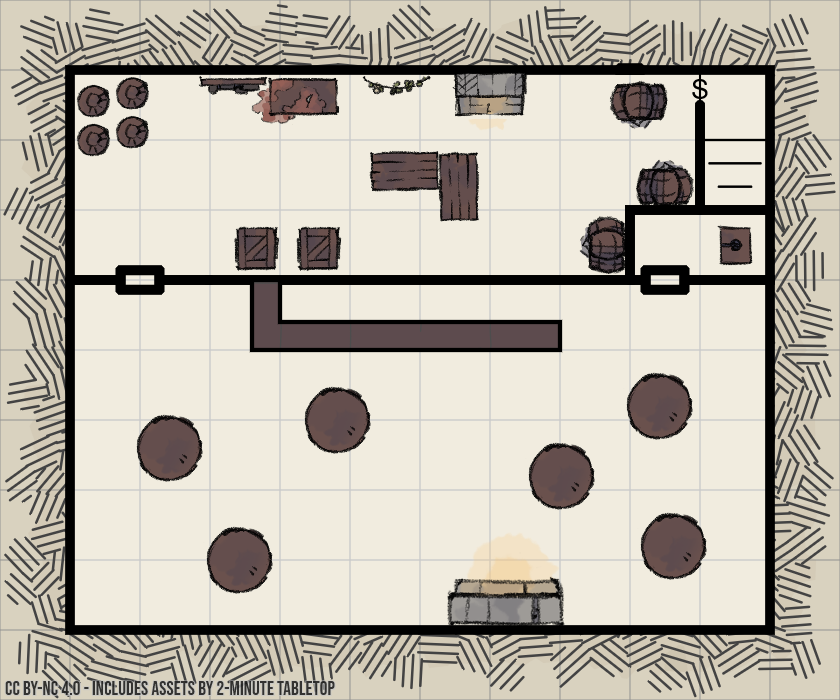
\includegraphics[height=.4\textheight]{assets/innUpstairs.png}
\end{figure*}
\begin{figure*}[ht]
  \centering
  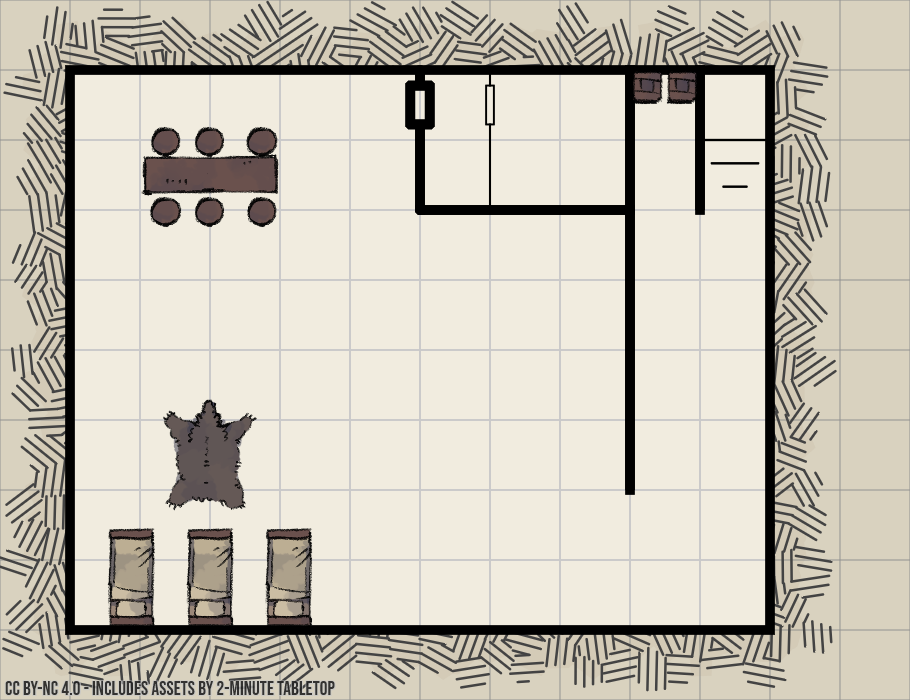
\includegraphics[height=.4\textheight]{assets/innDownstairs.png}
\end{figure*}

\DndArea{The Salty Swashbuckler Main Floor}
The tavern is only a single story tall.
The inside of the tavern is dimly lit and dirty.
As you enter, you can tell the door is not hung correctly and slams shut with a loud thud.
One man stands behind the counter and waves to the party as they enter.

\DndSubArea{The Barman}
If the party approaches him, the barman scrutinizes the group before speaking to them:

\begin{DndReadAloud}
  Ahh, you must be one of them there adventuring groups, huh?
  Phooey and folley, if you ask me, but if you're looking for a ship for work or travel I know a guy...
  Or is it just a drink you're after?
  I can imagine it's thirstin' work.
\end{DndReadAloud}

The barman is really the Carmine's lookout, though he does not initially suspect they have been found out.
If the party requests a drink he will serve them without further question and leave them to their table.

However, if the party starts to ask about the Carmines in any way, the barman will ``accidentally'' knock a glass bottle from the bar, shattering it to pieces.
This is a signal to the Carmines in the common room to make for the back room.
The two thieves use stealth to make their way to the back room and through the secret door.

If they are caught by a watchful party member, they choose to run for the secret door, yelling to ready the others in the basement
If they are not caught, the party will notice that their seats are empty.

\DndSubArea{Patron's Tables}
At the furthest left table, sit three men, two with red armbands.
If the party does not make any obvious actions towards them, they continue with their drinks for a short while.
Eventually one will stand up and make their way to the latrine.
Shortly after, the man returns pats his friend on the shoulder and motions that they should go.
Both say goodbye to the third man at the table, turn for the door to the backroom while nodding to the barman.

Shortly after that, the barman calls out that it is last call and everyone has fifteen minutes to get out or they get the boot.
All of the patrons groan collectively but start file out over the fifteen minute allotment.
Once the other patrons are gone the barman will attempt to shoo the party out, but now that the crowd has left, it is an opportune moment to question the barman.

He can be intimidated into telling the party about the back room with a DC 15 Charisma (Intimidation) check.
The barman can also be convinced to tell the party the hideout is in the basement with a DC 15/20 Charisma (Persuasion) check.
In both cases, the barman begs the party to let him go, claiming he has not had anything to do with the gang, he is just forced to stand watch for them.

\section{The Aftermath}
Gundren: I just can't wait, I need to leave now. I can't risk this.
A few days to settle their affairs and then follow them on the road.

\appendix
\chapter{Monsters}

\begin{DndMonster}{Thief}
  \DndMonsterType{Medium humanoid (any race), chaotic neutral}
  \DndMonsterBasics[
    armor-class=13,
    hit-points=\DndDice{4d8},
    speed={30 ft., climb 30ft.}
  ]
  \DndMonsterAbilityScores[str=8, dex=14, con=10, int=10, wis=12, cha=12]
  \DndMonsterDetails[
    skills={Stealth +6},
    senses={passive Perception 11},
    languages={Common, Thieves' Cant},
    challenge={1/4}
  ]
  
  \DndMonsterAction{Sneak Attack (1/turn)}
  The thief deals an extra \DndDice{1d6} damage when 
  \begin{enumerate*}[label={(\arabic*)}]
    \item it hits a target with a weapon attack and has advantage on the attack roll, or
    \item when the target is within 5 ft. of an ally of the thief that isn't incapacitated and the thief does not have disadvantage.
  \end{enumerate*}

  \DndMonsterSection{Actions}
  \DndMonsterMelee[
    name=Mace,
    mod=+0,
    reach=5,
    targets=one target,
    dmg=\DndDice{1d6-1},
    dmg-type=bludgeoning
  ]
  \end{DndMonster}

\end{document}
